\documentclass[border=2pt]{standalone}
\usepackage{tikz}
\begin{document}
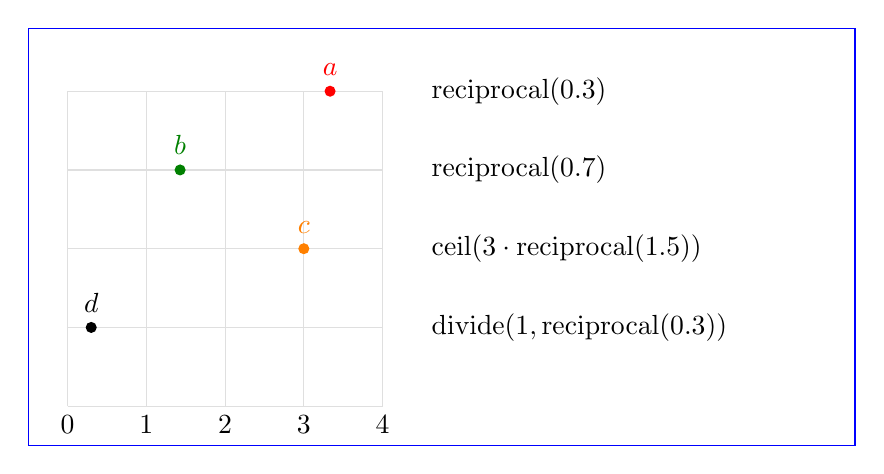
\begin{tikzpicture}
  \draw[blue] (-.5,-.5) rectangle (10,4.8);
  \draw[gray!25] (0,0) grid (4,4);
  \foreach \x in {0,1,2,3,4} \node[below] at (\x,0) {$\x$};
  \node[anchor=west] at (4.5,4) {reciprocal$(0.3)$};
  \node[anchor=west] at (4.5,3) {reciprocal$(0.7)$};
  \node[anchor=west] at (4.5,2) {ceil$(3\cdot\mathrm{reciprocal}(1.5))$};
  \node[anchor=west] at (4.5,1) {divide$(1,\mathrm{reciprocal}(0.3))$};
  \pgfmathsetmacro{\r}{reciprocal(0.3)}
  \fill[red] (\r,4) circle (2pt) node[above=2pt] {$a$};
  \fill[green!50!black] ({reciprocal(0.7)},3) circle (2pt) node[above=2pt] {$b$};
  \fill[orange] ({ceil(3*reciprocal(1.5))},2) circle (2pt) node[above=2pt] {$c$};
  \fill[black] ({divide(1,reciprocal(0.3))},1) circle (2pt) node[above=2pt] {$d$};
\end{tikzpicture}
\end{document}
